\documentclass[twocolumn]{article}
\usepackage[spanish]{babel}
\usepackage{caption}
\usepackage{graphicx}
\usepackage{amsmath}
\setlength{\parindent}{0pt}

\author{Josué Villasante}
\title{Potencia de un laser en función del ángulo de una lamina retardadora}

\begin{document}
	\maketitle

	\section{Procedimiento}
		El procedimiento fue muy similar al anterior. El haz de luz producido por el láser era polarizado, tuvo una potencia de 100mW y una longitud de onda de 405nm. Este fue reflejado 90$^{\circ}$ primero en un cubreobjetos y luego 90$^{\circ}$ en un espejo. El cubreobjetos permitió reducir la potencia del haz de luz a una aceptable por el medidor, pero produjo dos haces debido a que ambas superficies reflejan. Para eliminar uno de los haces de luz más adelante se utilizó un iris. Luego se colocó una lamina retardadora de media onda, un polarizador de tipo \emph{wire grid} y finalmente el medidor de potencia.

		\begin{center}
			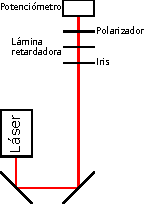
\includegraphics[width=100pt]{img/layout.pdf}
			\captionof{figure}{Esquemática del experimento.}
		\end{center}

		Para iniciar el experimento se colocó solo el polarizador, se encontró el ángulo de mínima potencia y se rotó 90$^{\circ}$ para así obtener la mayor potencia. Luego se colocó la lamina retardadora antes del polarizador y marcando 241$^{\circ}$ se empezó a medir la potencia cada 10$^{\circ}$ hasta llegar a 61$^{\circ}$. La lamina en total rotó 180$^{\circ}$.
	
	\section{Resultados}
		De los 19 puntos se observaron 3 picos de 966$\mu$W, 1324$\mu$W y 1241$\mu$W, y dos mínimos de 53.5$\mu$W y 46.3$\mu$W.

		\begin{center}
			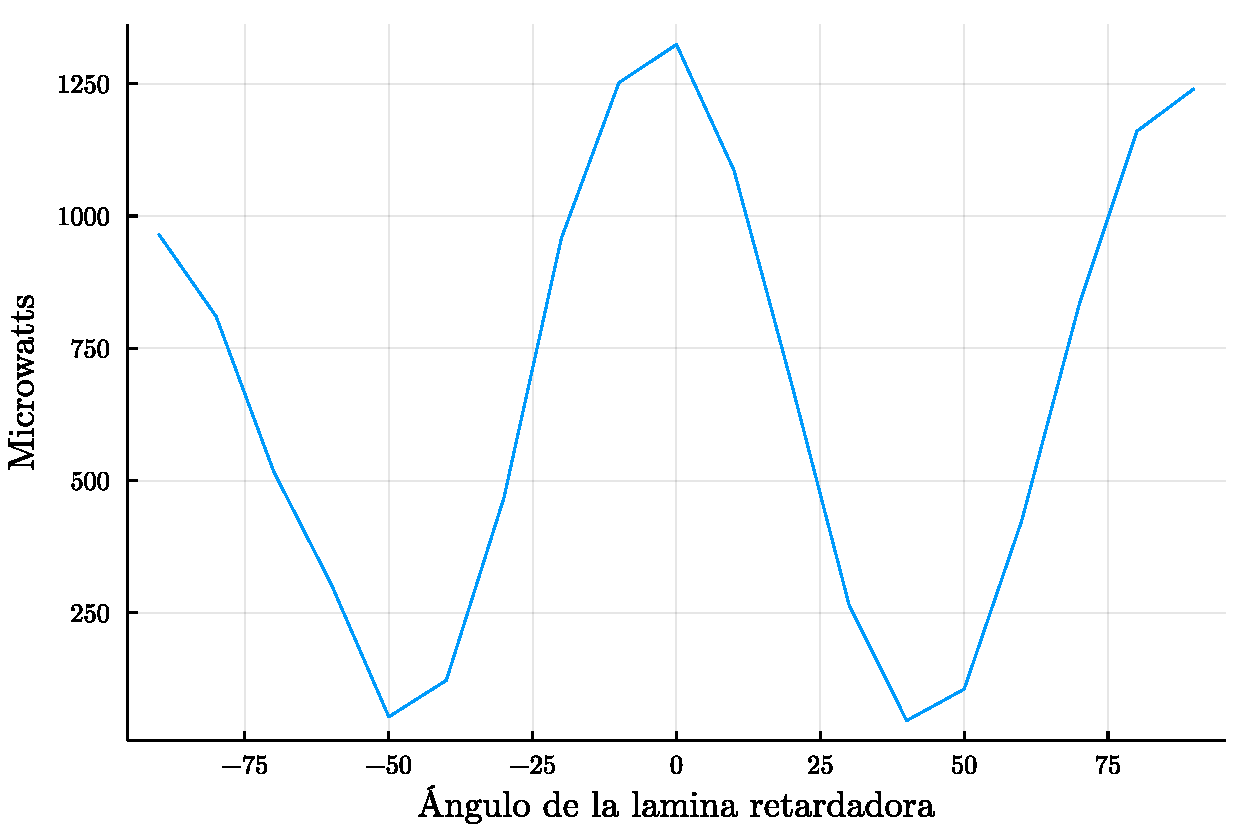
\includegraphics[width=230pt]{img/results.pdf}
			\captionof{figure}{Potencia medida en función del ángulo de la lamina retardadora.}
		\end{center}
	
	\section{Discusión}
		Vemos que a comparación del polarizador la potencia varía dos veces más \emph{rápida}. Por lo tanto, se puede decir la potencia en función del ángulo se ajusta a la siguiente función.

		$$
		P(x) = a \cos(\frac{1}{2}x)^2
		$$

		Tomando que $a=1324$, el máximo valor medido, vemos que se ajusta correctamente.

		\begin{center}
			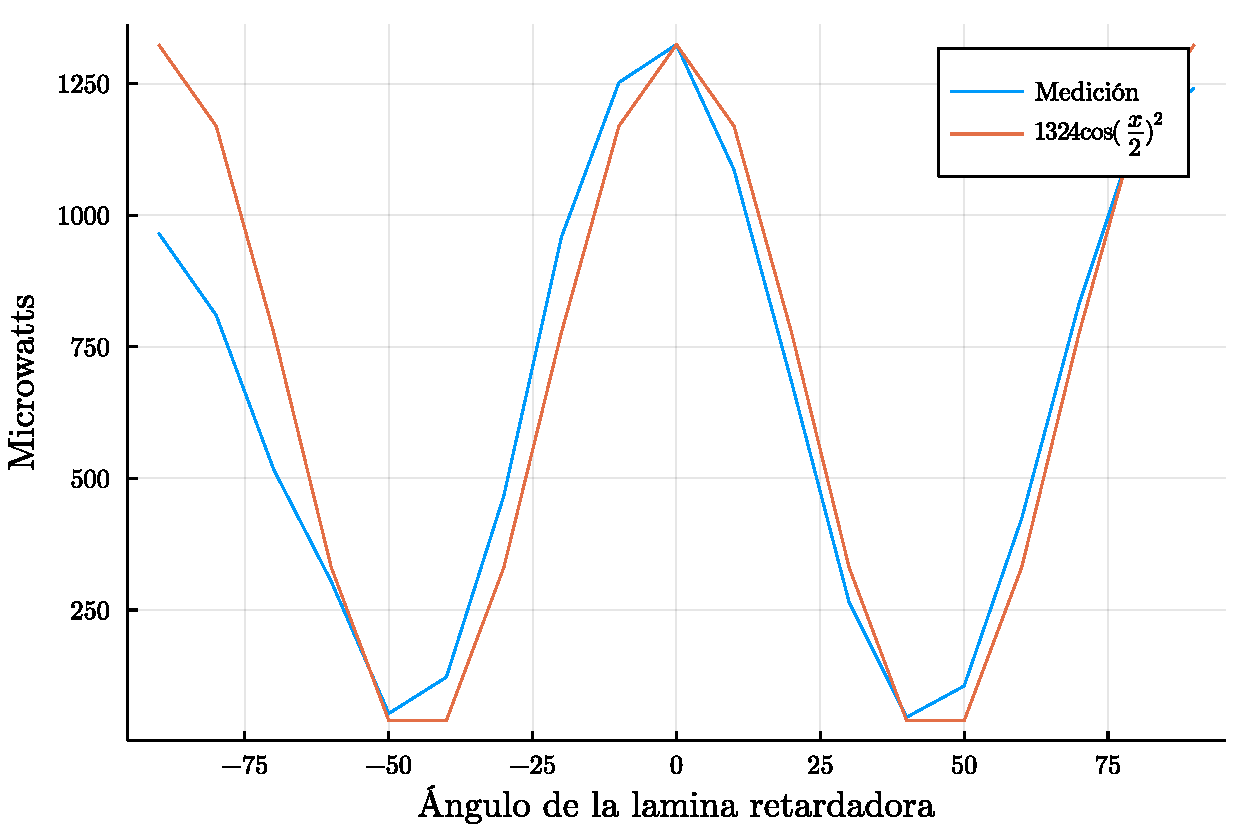
\includegraphics[width=230pt]{img/comparison.pdf}
			\captionof{figure}{Potencia medida en comparación con lo esperado.}
		\end{center}
\end{document}